\section{Data}

The dataset consists of images captured using a scanning electron microscope (SEM). These images are part of a study focused on the thickness of coating cladding layers applied to various materials, both before and after being subjected to high temperatures and aggressive environments, to assess the properties of these layers. The layers of interest are marked within red rectangular boxes in Figure~\ref{fig:three-images}. These layers exhibit varied characteristics, such as differences in color, number of layers, and degrees of damage.

\begin{figure}[ht]
    \centering
    \begin{subfigure}{0.3\textwidth}
        \centering
        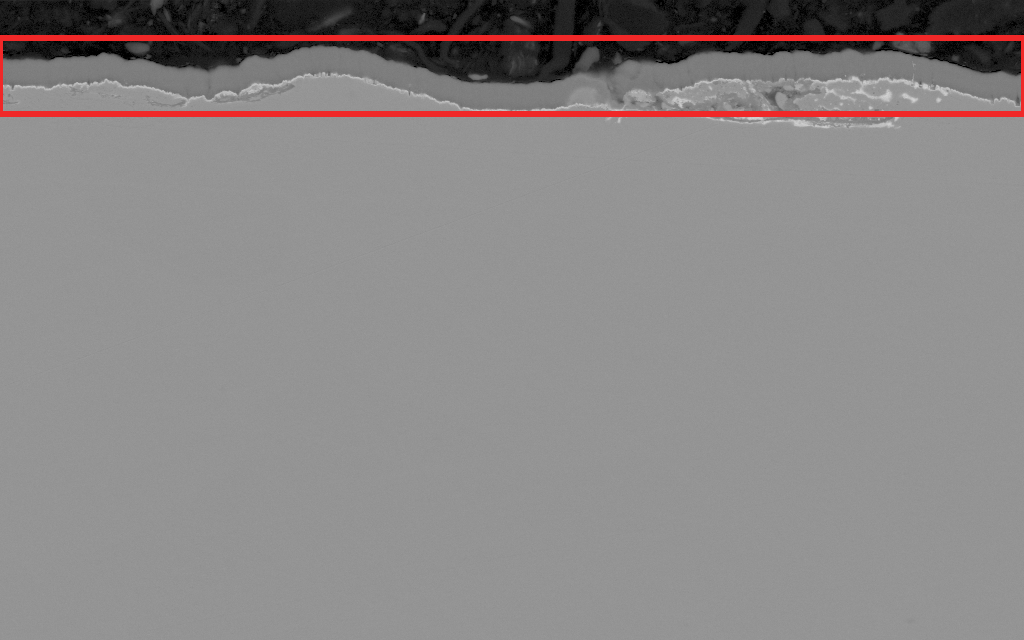
\includegraphics[width=\linewidth]{PICTURES/original_data/11.png}
        \label{fig:subfig1}
    \end{subfigure}
    \hfill
    \begin{subfigure}{0.3\textwidth}
        \centering
        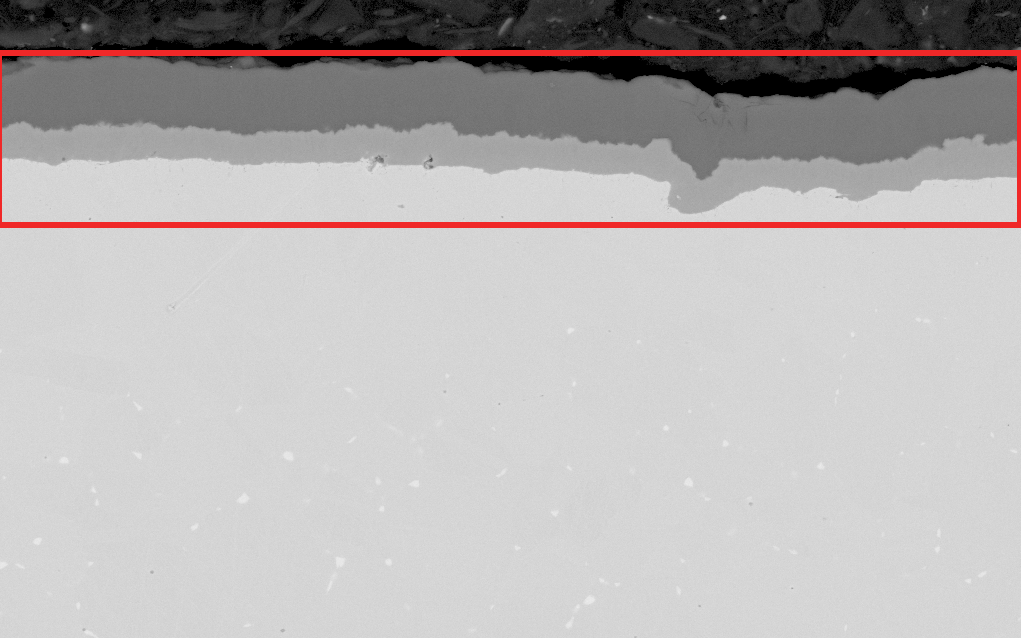
\includegraphics[width=\linewidth]{PICTURES/original_data/177.png}
        \label{fig:subfig2}
    \end{subfigure}
    \hfill
    \begin{subfigure}{0.3\textwidth}
        \centering
        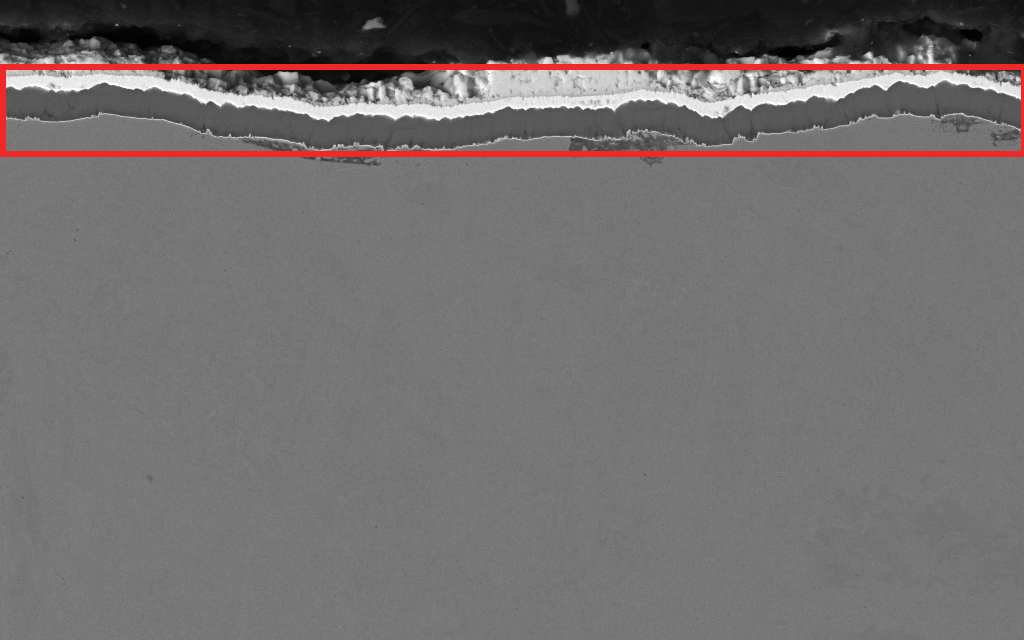
\includegraphics[width=\linewidth]{PICTURES/original_data/208.png}
        \label{fig:subfig3}
    \end{subfigure}
    \caption{SEM images with highlighted coating layers in red boxes.}
    \label{fig:three-images}
\end{figure}

\subsection{Manual Data Processing}\label{sec:ManualProc}

The images are initially obtained in *.tif format after the measurements with the SEM. Then they are processed using Fiji, an open-source image processing software that is a distribution of ImageJ \cite{Schindelin2012}. A predefined template consisting of 20 lines is used for measurements, each corresponding to a specific measurement region. The first ten lines, indexed 1 to 10, are employed to measure the thickness of the coating layer, while the second set of ten lines, located beneath the first, are used to measure oxidation. The lines are evenly distributed across the image's width and share a constant x-coordinate.

Subsequent to the initial measurements, each of the 20 lines is manually adjusted to align with either the oxidation or the coating layer. After all adjustments are completed, the measurements are exported to Excel for statistical analysis. If a layer is absent at the location of a predefined line, the line is left in its position but is later marked as 0.0 in the corresponding Excel spreadsheet. 

The images are grouped into batches of approximately 30, with each batch containing images of the same material, though different parts of the material are captured in each image, leading to a high degree of similarity among the images in each batch. The initial image of each batch typically takes longer to process since the line adjustments from the previous image are reused for the other images in the same batch. As the remaining images within a batch are more similar, they require less time for adjustment. The primary challenges arise in images where significant oxidation is present, which may destroy the coating layer.

Figure~\ref{fig:Fiji} illustrates the measurements performed in Fiji. Lines 1 to 10, used for measuring the coating layer, are shown. In this example, no oxidation layer is present.

\begin{figure}[H]
    \centering
    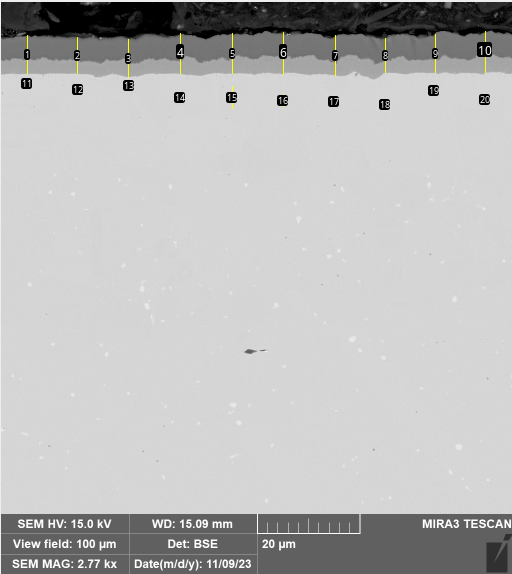
\includegraphics[width=0.7\linewidth]{PICTURES/625_Al2O3_3500h_low_cross_strana2_13_measurements.png}
    \caption{Measurement in Fiji software.}
    \label{fig:Fiji}
\end{figure}

\newpage
Although oxidation and coating layers are both critical for material characterization, this thesis focuses specifically on automating the measurement of coating layer thickness in SEM images. Coating layers prevent underlying materials from oxidizing, making oxidation layers less common in samples that feature coatings.


\subsection{Fiji Adjustments}\label{sec:1.2.2}

The first modification involved the customization of the `StartUpMacro` in Fiji, which runs automatically each time the program is launched. Three new buttons were incorporated into the interface: one for saving measurements, another for adjusting the scale, and a third for displaying the default lines.

The \texttt{Save Measurement} button was implemented to store data from the 20 lines required to create the dataset necessary for automation. This feature ensures that the required measurements are automatically saved.

The \texttt{Adjust Scale} button was added to streamline user interaction with Fiji, addressing the need to manually adjust the scale at the start of each session. Since the scale, visible at the bottom of the image, remains constant across all images, this functionality simplifies the process.

The \texttt{Set Default ROI} button was introduced to allow the researcher to quickly access the prepared default 20 lines for new batch.

Furthermore, the extraction of the final measured lengths into an Excel file was simplified.

\subsection{Dataset}

As previously mentioned, the first step in dataset creation was gathering data. Prior to this, results were stored exclusively in Excel tables, which included the lengths of the measurement lines but lacked positional information, rendering them insufficient for generating a comprehensive dataset. After collecting enough data thanks to the Fiji adjustments~\ref{sec:1.2.2}, stored in a zip folder containing 20 *.roi files (each representing one measurement line), the dataset was created.

\subsubsection{Polygon Labels}

The initial set of labels was generated using measured data from ten measurement lines. The upper ten points of each line were connected to form a boundary curve, and the same process was applied to the lower points. The space between these two curves was then filled to generate the mask. However, due to missing information at the edges of the image, cropping of both the images and the masks was needed. Figures~\ref{fig:polygon_sem_color} and~\ref{fig:polygon_sem} illustrate that the masks do not extend to the edges of the images.

This labeling process was automated using a Python script. The script loads each image along with the corresponding zip folder containing the line measurements. The x and y coordinates of these lines are stored in arrays, which are then mapped onto an Excel sheet. Any lines marked as missing (labeled as 0) in Excel are excluded, even if they are present in the folder.

To interpolate the boundary points, cubic spline interpolation \cite{fritsch1980monotone} was employed. The upper and lower boundary points, stored in arrays, were used to create a spline model, which was then applied to generate the boundary curve. The interpolation function was used with a smoothing parameter of s=0 to ensure that the interpolation closely followed the measured points. The space between the curves was filled, resulting in a binary mask. The mask was resized to match the original image dimensions and saved as a binary mask.

This approach enabled the automated generation of masks from the measured oxidation lines, ensuring that the labels were consistent with the scientific data.



\subsubsection{K-means Labels} \label{sec:kmeans}

The K-means algorithm \cite{lloyd1982least} is a clustering method used in unsupervised machine learning, designed to minimize a function that measures the quality of cluster formation. The algorithm selects $k$ random points as cluster centers from the dataset, assigning each data point to the nearest center based on distance. The geometric center of each cluster is then recalculated, and the process repeats until a convergence criterion is met.

K-means is particularly effective for images with distinct pixel colors. One of the key advantages of K-means is that it does not require prior labels, but the value of $k$ (the number of clusters) must be chosen carefully. Thus, the optimal $k$ was determined through testing for each batch of images.

In most cases, further processing was necessary, particularly to isolate the coating layer while eliminating noise. As illustrated in Figures~\ref{fig:kmean_sem_color} and~\ref{fig:kmean_sem}, K-means encountered difficulty distinguishing between oxidation and the coating layer, as their pixel values were similar and even formed a continuous cluster. Consequently, the algorithm alone was insufficient for accurately measuring the coating layer.

\subsubsection{K-means Refined}

To improve the accuracy of the K-means labels, the entire dataset was reviewed collaboratively with the researcher, and the masks were manually refined using image editing software. These manually refined masks, considered the most accurate, were validated by the researcher. The final version of the masks was then used as a test dataset for further automation.


\begin{figure}[ht]
    \centering
    \begin{subfigure}{0.3\textwidth}
        \centering
        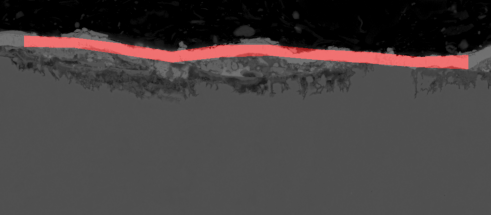
\includegraphics[width=\linewidth]{PICTURES/MASK/POLYGON316L_W_3500h_low_cross_strana1_07.png}
        \caption{Polygon mask}
        \label{fig:polygon_sem_color}
    \end{subfigure}
    \hfill
    \begin{subfigure}{0.3\textwidth}
        \centering
        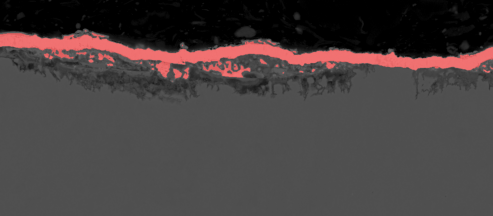
\includegraphics[width=\linewidth]{PICTURES/MASK/KMEAN316L_W_3500h_low_cross_strana1_07.png}
        \caption{K-Means mask}
        \label{fig:kmean_sem_color}
    \end{subfigure}
    \hfill
    \begin{subfigure}{0.3\textwidth}
        \centering
        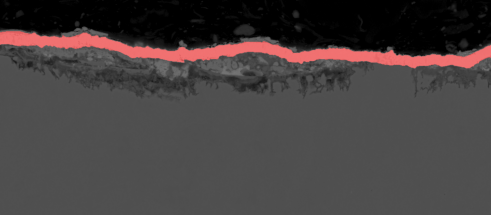
\includegraphics[width=\linewidth]{PICTURES/MASK/149_original.png}
        \caption{Refined K-Means}
        \label{fig:kmean_refined_color}
    \end{subfigure}
    \caption{Masks on SEM image}
    \label{fig:three-masks_color}
\end{figure}

\begin{figure}[ht]
    \centering
    \begin{subfigure}{0.3\textwidth}
        \centering
        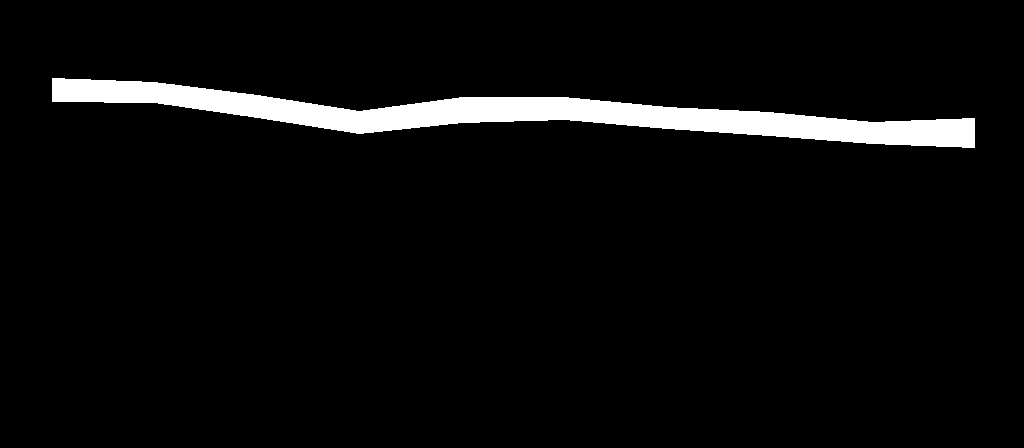
\includegraphics[width=\linewidth]{PICTURES/MASK/316L_W_3500h_low_cross_strana1_07(2).png}
        \caption{Polygon mask}
        \label{fig:polygon_sem}
    \end{subfigure}
    \hfill
    \begin{subfigure}{0.3\textwidth}
        \centering
        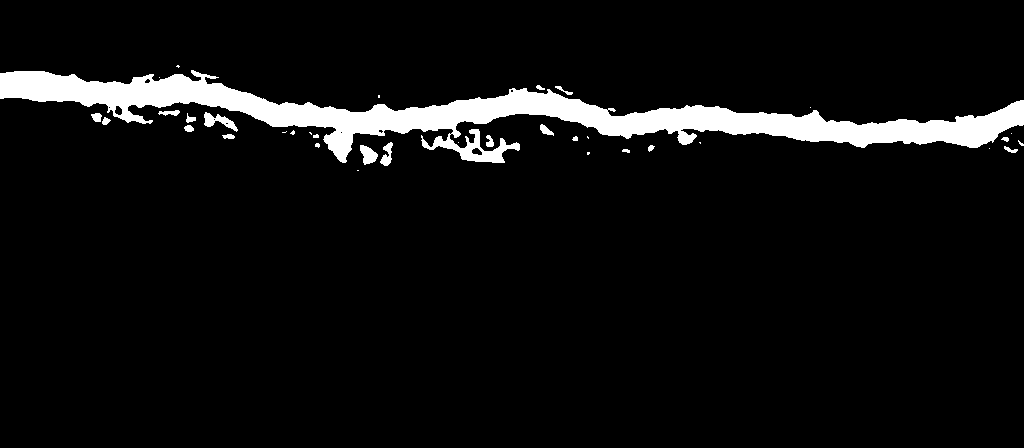
\includegraphics[width=\linewidth]{PICTURES/MASK/316L_W_3500h_low_cross_strana1_07.png}
        \caption{K-Means mask}
        \label{fig:kmean_sem}
    \end{subfigure}
    \hfill
    \begin{subfigure}{0.3\textwidth}
        \centering
        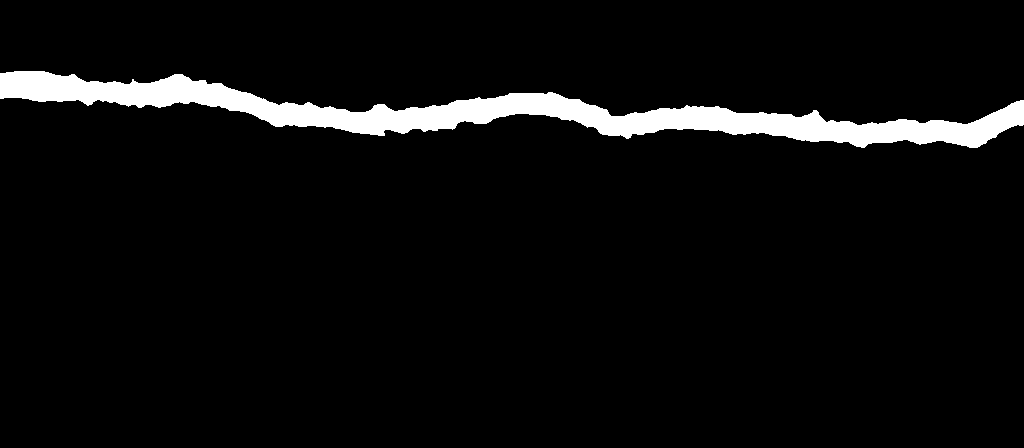
\includegraphics[width=\linewidth]{PICTURES/MASK/316L_W_3500h_low_cross_strana1_07(1).png}
        \caption{Refined K-Means}
        \label{fig:kmean_refined_sem}
    \end{subfigure}
    \caption{Binary masks}
    \label{fig:three-masks}
\end{figure}
